\documentclass{article}
\usepackage{ctex}  %使用宏包(为了能够显示汉字)
\title{乙醇偶合制备C4烯烃}  %文章标题
\author{}
\date{}
\usepackage{amsmath}
\usepackage{amssymb}
\usepackage{multirow}
\usepackage{longtable}
\usepackage{graphicx}
\usepackage{subfigure}
\usepackage{url}
\usepackage[a4paper,left=25mm,right=25mm,top=25mm,bottom=25mm]{geometry}  
\newcommand{\enabstractname}{Abstract}
\newcommand{\cnabstractname}{摘要}
\newenvironment{enabstract}{%
	\par\small
	\noindent\mbox{}\hfill{\bfseries \enabstractname}\hfill\mbox{}\par
	\vskip 2.5ex}{\par\vskip 2.5ex}
\newenvironment{cnabstract}{%
	\par\small
	\noindent\mbox{}\hfill{\bfseries \cnabstractname}\hfill\mbox{}\par
	\vskip 2.5ex}{\par\vskip 2.5ex}
\usepackage{listings}

\begin{document}
	\maketitle
	\begin{cnabstract}
		此次数学建模我们要探究的是在乙醇偶合制备C4烯烃的过程中催化剂组合与温度对反应的影响。我们需要考虑乙醇转化率以及C4烯烃选择性等因素,建立此化学问题的数学模型并设计相应算法,得到不同变量间的相互关系,并设计合适的实验进行更深入的探究。
		
		在第一个问题中,我们首先探究了给定催化剂条件下,不同温度对于乙醇转化率、C4烯烃选择性的影响,主要通过回归理论分析了附件1中给出的数据,最终拟合确定了二次多项式的函数关系。在对各组数据进行分析得到多项式系数后,我们进行了显著性分析,证明了模型的合理性。其次,我们对附件2中实验数据进行处理,并主要从化学机理的角度,探究了时间对于该化学反应的影响。
		
		在第二个问题中,我们需要探究催化剂组合和温度对乙醇转化率与C4烯烃选择性的影响。我们首先对数据进行了预处理,将催化剂组合拆分成了多个连续型或离散型变量。其次,我们应用相关性分析理论,通过SPSS对各变量进行了偏相关分析,得到了相关性系数和相应的拒绝假设概率,初步确定了各变量间的关系。接着,我们采取控制变量的方法,将各变量分离成多组,分别进行定性或定量分析,探究其对反应的影响。在得到控制变量方法的结果后,我们发现变量间并非单一的影响关系,因此引入了神经网络作为计算系统。我们建立了三层的BP神经网络,对数据进行了训练和检验,更加准确地模拟出了各变量之间的关系。
		
		在第三个问题中,为了使得C4烯烃收率尽可能高,我们需要确定合适的催化剂组合与温度,因此建立了优化模型。根据我们此前已建立的神经网络模型,我们采取遗传算法对数据进行搜索,得到了相应的局部较优解,分别给出了温度无特殊条件限制和温度低于350度时的最佳催化剂组合与温度。
		
		在第四个问题中,为了验证上一问题中解的合理性,我们基于控制变量的思想,分别改变了某一特定变量,设计了五组实验,并且在神经网络模型和遗传算法的基础上预测了实验的可能结果。
		
		最后,我们在论文末尾对文章中模型和算法的可行性进行了补充分析与说明。同时,我们总结了模型和算法的优缺点,并初步给出了改进策略。至此,本篇文章正文部分结束,附录部分我们给出了文章的支撑材料。
		
		\par\textbf{关键字:回归分析、相关性分析、控制变量、神经网络算法、遗传算法} 
	\end{cnabstract}
	
	\newpage
	\section{情景概述}
	乙醇是生产制备重要化工产品C4烯烃的原料。在制备过程中,催化剂组合和温度对C4烯烃的选择性和C4烯烃收率有着一定程度的影响。此次问题的场景便是对催化剂组合进行设计并在不同温度下进行一系列实验,要求对上述实验的结果进行分析和探讨,找出各变量对本反应的影响关系。通过建立数学模型和分析实验数据,得出最适催化剂组合和温度条件用于实际制备工艺,并能够在特定条件下进行一定程度的预测来给出合适的实验条件和方案。在进行上述分析后,选取合适范围改变各变量设计更具体深入的实验。
	
	\section{基本假设}
	\begin{itemize}
		\item[(1)]文章中所有实验数据均真实可靠。
		\item[(2)]文章中所有参数设置的范围阈值都依据实验所给数据建立。
		\item[(3)]文章中设计的算法和实验方案都能用于题干场景。
	\end{itemize}

	\section{变量声明}
	\begin{table}[!h]
		\centering
		\caption{模型所需变量}
		\begin{tabular}{|l|l|}
			\hline
			变量 & 变量名 \\
			\hline
			乙醇转化率          & $CR$  \\
			C4烯烃选择性        & $ST$  \\
			C4烯烃收率         & $PY$  \\
			温度             & $T_c$  \\
			时间             & $t$   \\
			催化剂组合          & $X$   \\
			催化剂质量和         & $x_1$  \\
			Co/SiO2和HAP装料比 & $x_2$  \\
			Co负载量          & $x_3$  \\
			乙醇浓度           & $x_4$  \\
			装料方式           & $x_5$ \\
			\hline
		\end{tabular}
	\end{table}

	\section{第一问}
	\subsection{回归理论}
	在分析两个变量的关系时,回归分析是一种很有效的定量分析方法。以多项式回归为例,假设$x$为自变量,$y$为因变量,它们之间的关系如下:
	\begin{equation}
		y=\beta_0 +\beta_1 x+\beta_2 x^2+\cdots+\beta_p x^p+\epsilon
	\end{equation}
	该式即为回归方程,其中$p$为已知的多项式次数,$\beta_i(i=1,2,\dots,p)$为未知的系数。假设已有$n$组关于$(x,y)$的值,回归即要选取$\beta_i$使$Q=\sum_{i=1}^n(y_i-\beta_0 -\beta_1 x-\beta_2 x^2-\cdots-\beta_px^p)^2$最小。通过最小二乘法可以得到使该关系式最小的$\hat{\beta_0},\hat{\beta_1},\dots,\hat{\beta_p}$作为系数值。这样便确立了回归方程,通过回归方程得到的每点估计值为$\hat{y_i}=\hat{\beta_0}+\hat{\beta_1}x_i+\cdots+\hat{\beta_p}x_i^p$。
	但关于数据与回归方程是否适合,需要做一定的评价与假设检验。评价回归方程的指标为决定系数$R^2$,表达式如下:
	\begin{equation}
		R^2=\frac{\sum_{i=1}^n(\hat{y_i}-\overline{y})^2}{\sum_{i=1}^n(y_i-\overline{y})^2}
	\end{equation}
	$R^2$越接近于1,说明数值点在回归曲线附近越密集,该回归的拟合度越好。另外,回归模型需要做一定的显著性检验。借用MATLAB中的Regress函数,它可以帮助我们对回归作F检验,得到F值以及拒绝回归假设的概率$p$。由于Regress函数中默认显著性水平值$\alpha$为0.05,一般$p<0.05$的回归被认为是可以通过显著性检验的。
	\subsection{乙醇转化率与温度关系分析}
	第一问首先要求我们在每种固定催化剂组合下研究乙醇转化率与温度的关系。对此我们通过回归分析的方法给这种关系作一个简单的定量分析。由附录中的实验数据,每种固定催化剂组合下只进行了5-7组不同温度的实验。对这些数据进行拟合的有关尝试,我们确立了运用多项式函数来进行回归分析。由于数据并不多,3次以上的函数容易出现过拟合的情况,而在实际的化学分析中也往往是用一次或二次关系式来刻画转化率与温度的关系。所以在此我们对数据进行一次和二次多项式回归的尝试,回归的关系表达式如下:
	\begin{equation}
		CR=a_1T_c+a_2,CR=b_1T_c^2+b_2T_c+b_3
	\end{equation}

	将转化率$CR$视为因变量$y$,温度$T_c$视为自变量$x$,以A1的催化剂组合为例,可以得到回归后的曲线拟合图以及相应的残差图如下所示:
	\begin{figure}[!h]
		\centering 
		\subfigure[一次回归$R^2=0.932$]{
			\label{Fig.sub.1}
			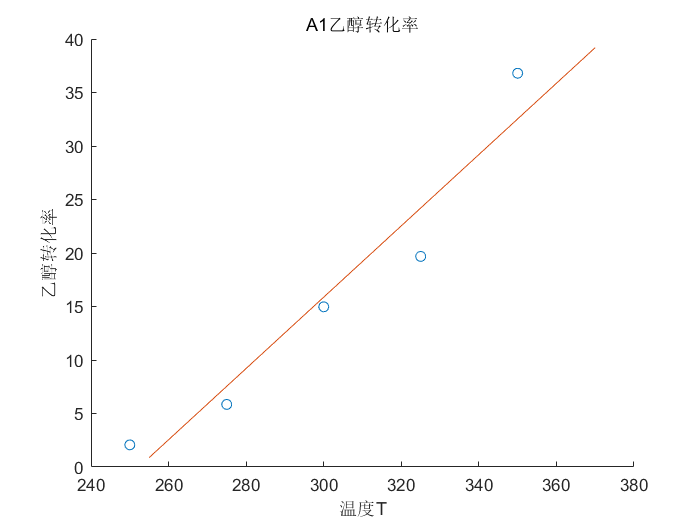
\includegraphics[width=0.45\textwidth]{A1-1.png}}
		\subfigure[二次回归$R^2=0.980$]{
			\label{Fig.sub.2}
			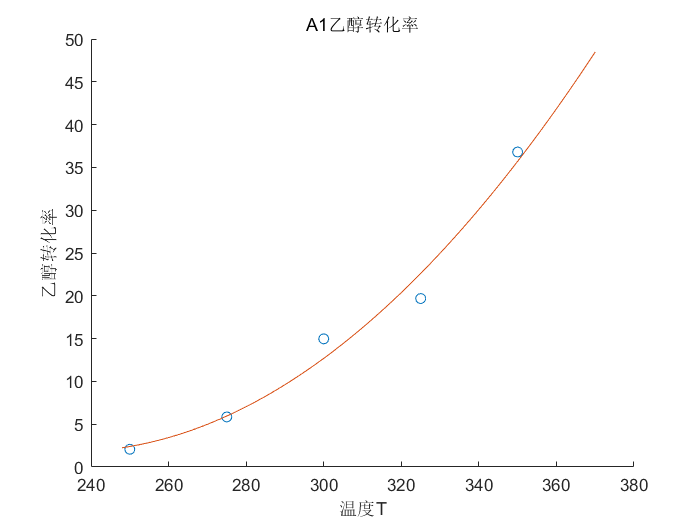
\includegraphics[width=0.45\textwidth]{A1-2.png}}
		\caption{乙醇转化率回归图}
	\end{figure}
	
	\begin{figure}[!h]
		\centering 
		\subfigure[一次回归残差]{
			\label{Fig.sub.1}
			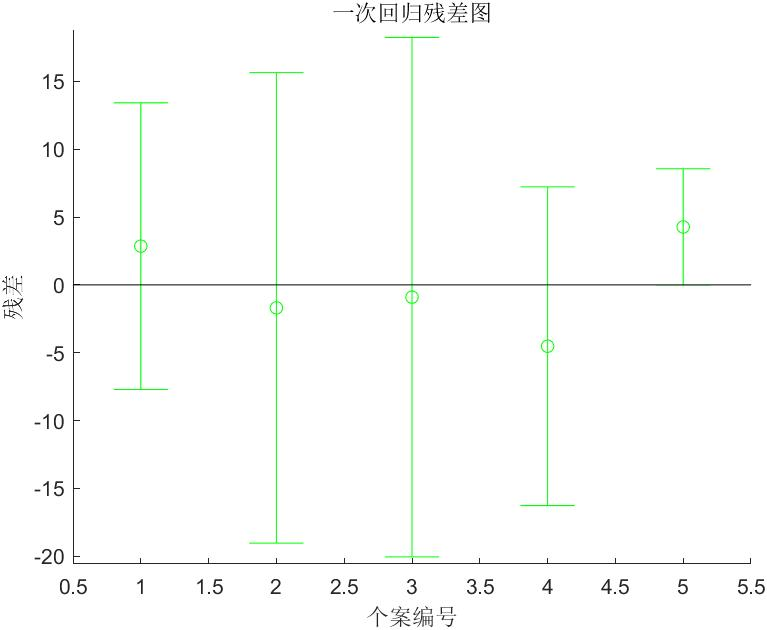
\includegraphics[width=0.45\textwidth]{一次回归残差1.jpg}}
		\subfigure[二次回归残差]{
			\label{Fig.sub.2}
			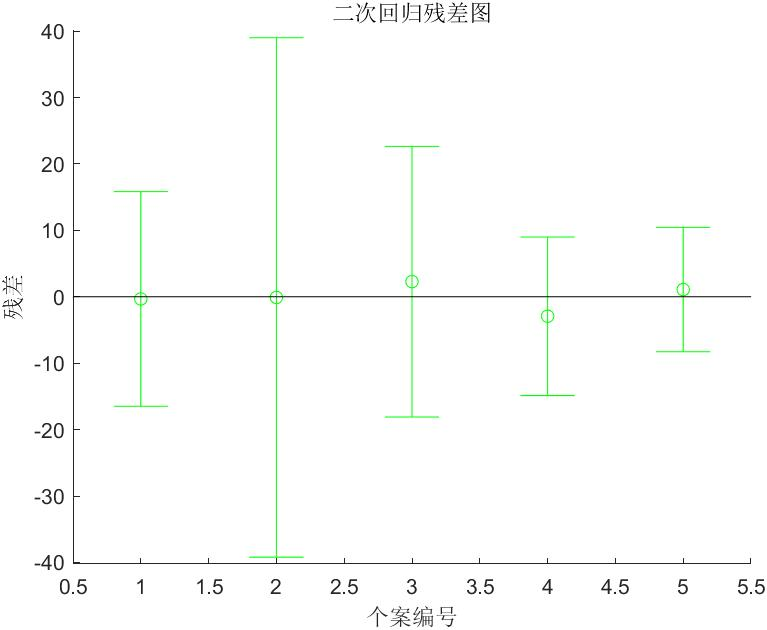
\includegraphics[width=0.45\textwidth]{二次回归残差1.jpg}}
		\caption{乙醇转化率回归残差图}
	\end{figure}
	
	\newpage
	通过对比二者的决定系数大小以及残差与零点的接近程度,可以确定用二次回归相比于一次会更好。下表便是由二次多项式回归确定的多项式系数和相应的回归检验参数。系数值通过定量的方式便给出了乙醇转化率与温度的关系。其中大部分能通过假设检验,说明回归合理。
	\begin{table}[!h]
		\centering
		\caption{乙醇转化率拟合结果}
		\begin{tabular}{|c|c|c|c|c|c|}
			\hline
			& \multicolumn{5}{c|}{乙醇转化率}                                          \\ \cline{2-6} 
			\multirow{-2}{*}{催化剂组合}    & 二次项系数   & 一次项系数    & 常数项       & 决定系数$R^2$ & 拒绝假设概率$p$ \\ \hline
			A1                         & 0.0025  & -1.1939  & 141.8074  & 0.9797                   & 0.0203  \\ \hline
			A2                         & -0.0007 & 1.1059   & -227.4149 & 0.9911                   & 0.0089  \\ \hline
			A3                         & -0.0003 & 0.6468   & -134.1885 & 0.9663                   & 0.0011  \\ \hline
			A4                         & 0.0004  & 0.3488   & -107.6114 & 0.9663                   & 0       \\ \hline
			A5                         & 0.0012  & -0.5624  & 72.7734   & 0.994                    & 0.0005  \\ \hline
			A6                         & 0.0017  & -0.5773  & 51.0045   & 0.9859                   & 0.0141  \\ \hline
			A7                         & -0.0003 & 0.551    & -102.3299 & 1                        & 0       \\ \hline
			A8                         & 0.0018  & -0.8029  & 97.1626   & 1                        & 0       \\ \hline
			A9                         & 0.0024  & -1.3475  & 187.1003  & 0.9905                   & 0.0095  \\ \hline
			A10                        & 0.0018  & -0.9864  & 135.5131  & 0.9939                   & 0.0061  \\ \hline
			A11						   & 0.0023  & -1.2735  & 177.778   & 0.9871                   & 0.0129  \\ \hline
			A12                        & 0.0019  & -0.9506  & 120.9377  & 1                        & 0       \\ \hline
			A13                        & 0.0022  & -1.2043  & 163.4118  & 0.9963                   & 0.0037  \\ \hline
			A14                        & 0.0022  & -1.0826  & 137.8797  & 0.9971                   & 0.0029  \\ \hline
			B1                         & 0.0019  & -0.9503  & 121.4967  & 0.9989                   & 0.0011  \\ \hline
			B2                         & 0.0025  & -1.3661  & 188.5082  & 0.9915                   & 0.0085  \\ \hline
			B3                         & 0.0025  & -1.3661  & 188.5082  & 0.9916                   & 0.0008  \\ \hline
			B4                         & 0.0021  & -1.1267  & 154.85    & 0.9867                   & 0.0015  \\ \hline
			B5                         & 0.0025  & -1.33524 & 185.3143  & 0.9916                   & 0.0008  \\ \hline
			B6                         & 0.0028  & -1.4441  & 190.0457  & 0.9904                   & 0.0009  \\ \hline
			B7                         & 0.0033  & -1.711   & 228.7107  & 0.9966                   & 0.0002  \\ \hline
		\end{tabular}
	\end{table}

	\newpage
	\subsection{C4烯烃选择性与温度关系分析}
	对于C4烯烃选择性,与前分析一致,我们也对数据进行一次和二次多项式回归的尝试,回归的关系表达式如下:
	\begin{equation}
		ST=a_1T_c+a_2,ST=b_1T_c^2+b_2T_c+b_3
	\end{equation}

	同样以A1的催化剂组合为例,可以得到回归后的曲线拟合图以及相应的残差图如下所示:
	\begin{figure}[!h]
		\centering 
		\subfigure[一次回归$R^2=0.787$]{
			\label{Fig.sub.1}
			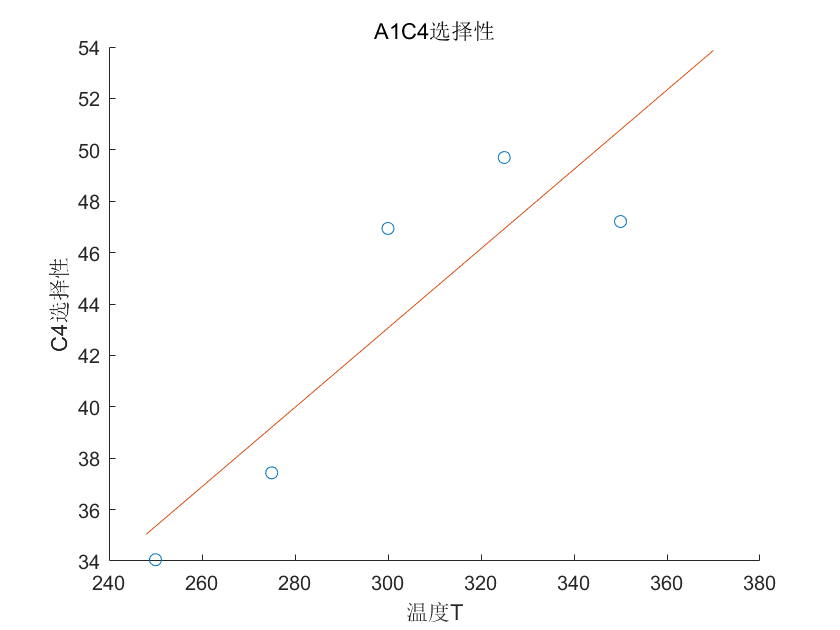
\includegraphics[width=0.45\textwidth]{A1-3.png}}
		\subfigure[二次回归$R^2=0.916$]{
			\label{Fig.sub.2}
			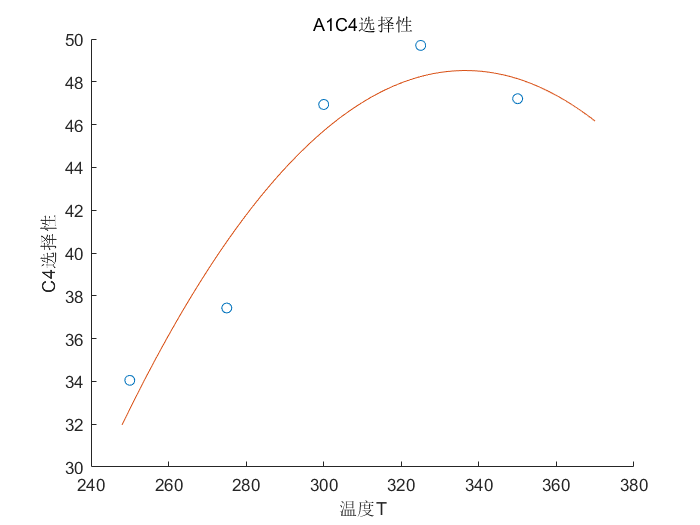
\includegraphics[width=0.45\textwidth]{A1-4.png}}
		\caption{C4烯烃选择性回归图}
	\end{figure}
	
	\begin{figure}[!h]
		\centering 
		\subfigure[一次回归残差]{
			\label{Fig.sub.1}
			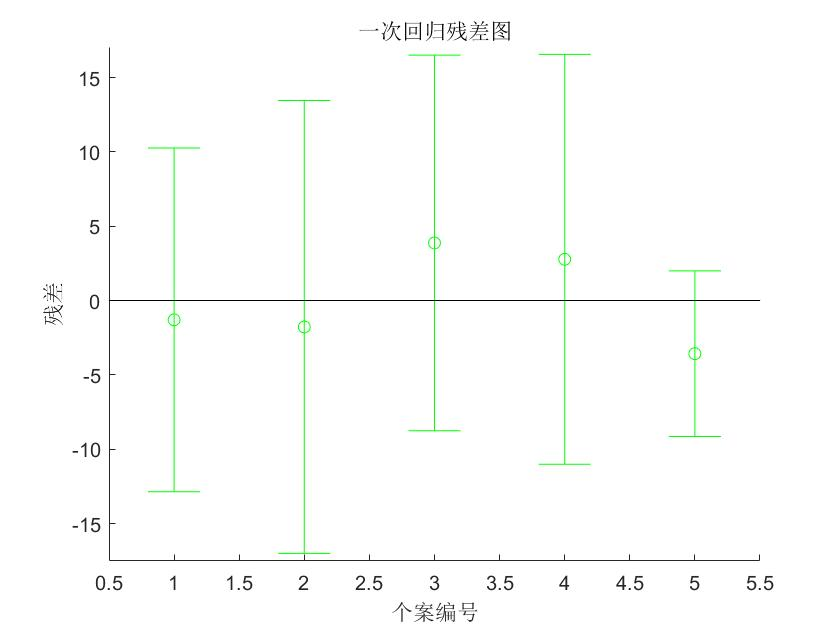
\includegraphics[width=0.45\textwidth]{一次回归残差2.jpg}}
		\subfigure[二次回归残差]{
			\label{Fig.sub.2}
			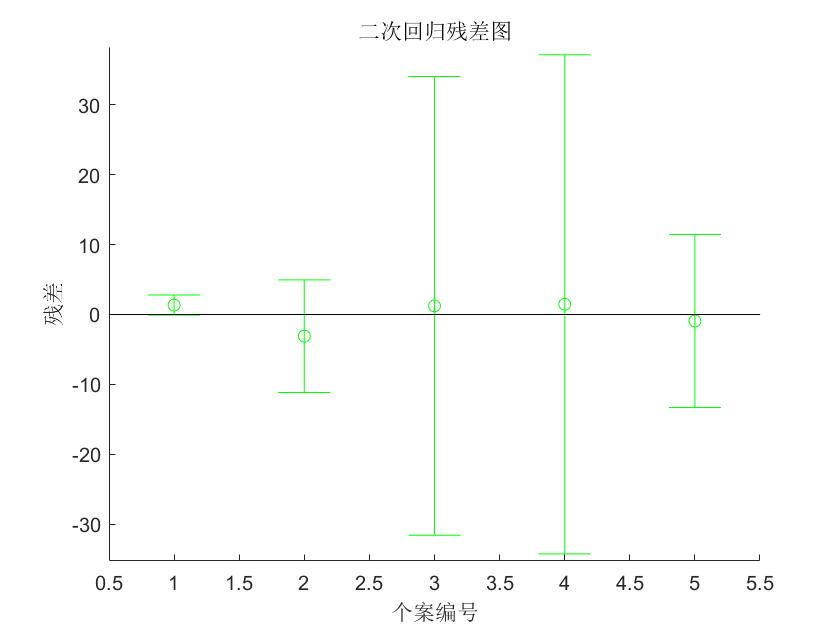
\includegraphics[width=0.45\textwidth]{二次回归残差2.jpg}}
		\caption{C4烯烃选择性回归残差图}
	\end{figure}
	
	\newpage
	对比二者的决定系数大小以及残差与零点的接近程度,可以确定用二次回归相比于一次会更好。下表是由二次多项式回归确定的多项式系数和相应的回归检验参数。系数值通过定量的方式便给出了C4烯烃选择性与温度的关系。其中大部分能通过假设检验,说明回归合理。
	\begin{table}[!h]
		\centering
		\caption{C4烯烃选择性拟合结果}
		\begin{tabular}{|c|c|c|c|c|c|}
			\hline
			& \multicolumn{5}{c|}{C4烯烃选择性}                                       \\ \cline{2-6} 
			\multirow{-2}{*}{催化剂组合}    & 二次项系数   & 一次项系数   & 常数项       & 决定系数$R^2$ & 拒绝假设概率$p$ \\ \hline
			A1                         & -0.0021 & 1.4222  & -190.7834 & 0.916                    & 0.084   \\ \hline
			A2                         & 0.0031  & -1.6463 & 234.7454  & 0.9803                   & 0.0194  \\ \hline
			A3                         & -0.0009 & 0.9244  & -171.0759 & 0.9551                   & 0.002   \\ \hline
			A4                         & 0.0012  & -0.5624 & 72.7734   & 0.9173                   & 0.0026  \\ \hline
			A5                         & 0.0011  & -0.4995 & 57.8837   & 0.9401                   & 0.0014  \\ \hline
			A6                         & 0.0022  & -1.2336 & 176.6157  & 0.9454                   & 0.0546  \\ \hline
			A7                         & 0.0012  & -0.5651 & 7407810   & 1                        & 0       \\ \hline
			A8                         & 0.0007  & -0.2446 & 19.819    & 1                        & 0       \\ \hline
			A9                         & 0.0001  & 0.218   & -53.4302  & 0.9949                   & 0.0051  \\ \hline
			A10                        & 0.0007  & -0.4036 & 59.7113   & 0.9785                   & 0.0215  \\ \hline
			A11						   & 0.0002  & -0.0675 & 5.5858    & 1                        & 0       \\ \hline
			A12                        & 0.0009  & -0.3829 & 45.3248   & 1                        & 0       \\ \hline
			A13                        & -0.0003 & 0.3425  & -64.3329  & 0.9768                   & 0.0015  \\ \hline
			A14                        & 0.001   & -0.494  & 64.8629   & 1                        & 0       \\ \hline
			B1                         & 0.0009  & -0.3654 & 39.0678   & 0.9989                   & 0.0011  \\ \hline
			B2                         & 0.001   & -0.4028 & 41.3295   & 0.9977                   & 0.0023  \\ \hline
			B3                         & 0.0005  & -0.1903 & 20.9699   & 0.9763                   & 0.0036  \\ \hline
			B4                         & 0.001   & -0.5487 & 81.074    & 0.9737                   & 0.0043  \\ \hline
			B5                         & 0.0006  & -0.2761 & 32.4024   & 0.9982                   & 0.0001  \\ \hline
			B6                         & 0.0003  & -0.0217 & -12.1287  & 0.9709                   & 0.005   \\ \hline
			B7                         & 0.0005  & -0.06   & -9.8584   & 0.9971                   & 0.0002  \\ \hline
		\end{tabular}
	\end{table}


	\newpage
	\subsection{时间对于化学反应影响的分析}
	根据附件2中的测试数据,我们作出了在350度、给定催化剂组合条件下,各变量随反应时间的变化示意图。
	\begin{figure}[!h]
		\centering 
		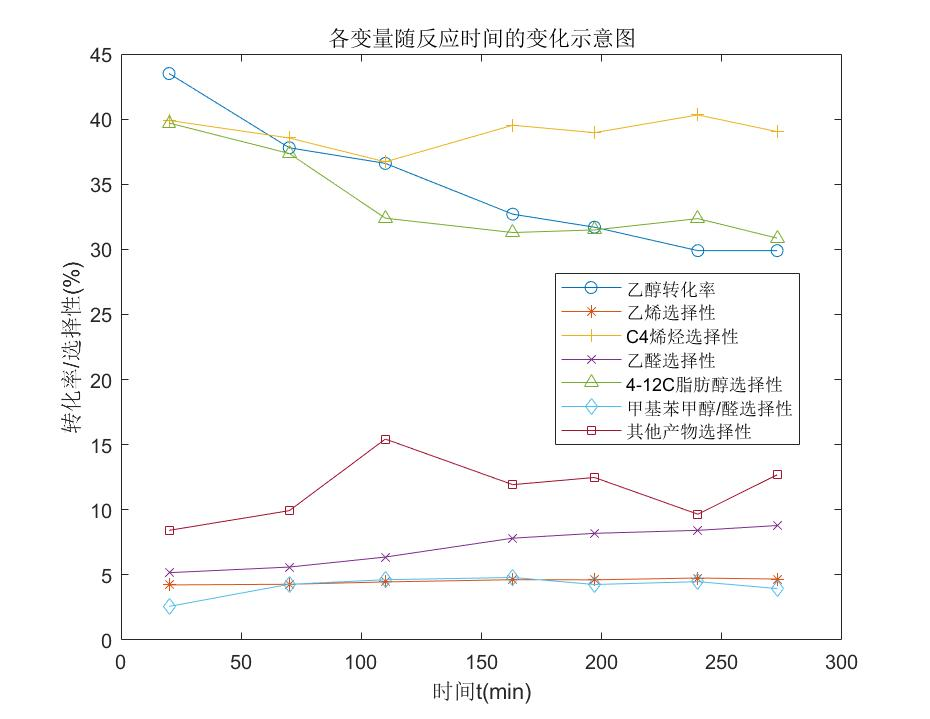
\includegraphics[width=0.6\textwidth]{timefigure.jpg}
		\caption{变量-时间测试结果图}
	\end{figure}
	
	从图表中可以看出,乙醇转化率随着时间增加而呈不断下降趋势。这是由于本反应为管道反应,随着时间增加,催化剂的活性降低,导致该反应进程的速率下降,从而单位时间内乙醇的瞬时转化率降低。
	
	另一方面,由于实验时温度始终保持不变,因此该反应的限度几乎不随时间发生变化,因此选择性的变化程度很小。

	\section{第二问}
	\subsection{变量预处理}
	在探讨不同催化剂组合及温度对乙醇转化率及C4烯烃选择性大小的影响前,我们先要确立催化剂组合是由哪些变量组成的。根据题目要求及具体数据,我们分析认为催化剂中催化剂质量总和、$Co/SiO_2$和HAP装料比(比值)、Co负载量、乙醇浓度(流量)以及催化剂的装料方式都在催化剂组合中对乙醇转化率及C4烯烃选择性大小构成了一定影响,而它们之间又是相互独立的。将催化剂总体视为变量$X$,这几个分离变量视为$x_i$,$X=(x_1,x_2,x_3,x_4,x_5)$即表示催化剂组合,任何$x_i$数值的不同代表了催化剂的不同(其中$x_1\sim x_4$都是具体数值,$x_5=1$表示装料方式1,$x_5=2$表示装料方式2)。
	
	确立了催化剂的变量组合,我们可以用一系列数据集来表示$A1\sim A14$及$B1\sim B7$的各催化剂组合。但其中有一个例外,它便是A11,该组合用的催化剂为石英砂,而非HAP。比较A11与A12,我们发现它们二者的区别仅在于催化剂种类不同,相同温度下,A11组中的乙醇转化率小于A12组,C4烯烃选择性更是远小于。观察发现,使用石英砂反应中乙醛选择性较大,从化学角度看,显然使用石英砂将更多催化乙醇,这与我们的目标不太相符。综合这两点理由,我们认为该题中不需要考虑石英砂作催化剂,仅需考虑以HAP为催化剂时的各催化剂组合变量的相关影响。
	
	综合催化剂变量与温度变量,探究影响关系即要确定函数关系:
	\begin{equation}
		CR=f(X,T_c)=f(x_1,x_2,x_3,x_4,x_5,T_c)
	\end{equation}
	\begin{equation}
		ST=g(X,T_c)=g(x_1,x_2,x_3,x_4,x_5,T_c)
	\end{equation}

	$CR-T_c$及$ST-T_c$的关系在第一问中已有初步讨论,本问中会更多关注催化剂$X$与$CR$、$ST$的关系。
	\subsection{相关性分析}
	相关性分析是一种判断两个或多个变量之间统计学关联的分析方法。对于可以连续取值的变量,可以用Pearson相关系数来判断两个连续变量之间的线性关联程度。对于连续变量$x$和$y$,其Pearson相关系数用$r$表示,表达式如下:
	\begin{equation}
		r=\frac{\sum_{i=1}^n(x_i-\overline{x})(y_i-\overline{y})}{\sqrt{\sum_{i=1}^n(x_i-\overline{x})^2\sum_{i=1}^n(y_i-\overline{y})^2}}
	\end{equation}
	其中检验用$t$统计量,同样引入显著性水平$\alpha$和拒绝假设概率$p$,当$p<\alpha$时认为该统计显著,即两变量存在线性相关性。
	
	许多情况下,变量数据很多,研究两变量间关系需要排除其余变量的影响,这就要用到偏相关理论。假设有$x_1$、$x_2$、$x_3$共3个变量,其中$x_3$为可控变量,下面计算除去$x_3$后$x_1$与$x_2$的偏相关系数,记为$r_{12,3}$,表达式如下:
	\begin{equation}
		r_{12,3}=\frac{r_{12}-r_{13}r_{23}}{\sqrt{1-r_{13}^2}\sqrt{1-r_{23}^2}}
	\end{equation}

	对于多个变量也可以类似求偏相关系数。在本题情境下,温度$T_c$与催化剂组合$X$中$x_1,x_2,x_3,x_4$均为连续型变量,而装料方式$x_5$为两个分立值,不适用该相关性分析。将数据导入SPSS软件,对于温度和催化剂相关变量进行对乙醇转化率和C4烯烃选择性的偏相关分析,得到相关性系数和相应的拒绝假设概率,如下表所示。
	\begin{table}[!h]
		\centering
		\caption{变量相关性分析}
		\begin{tabular}{|c|c|c|c|c|}
			\hline
			\multirow{2}{*}{变量} & \multicolumn{2}{c|}{乙醇转化率} & \multicolumn{2}{c|}{C4烯烃选择性} \\ \cline{2-5} 
			& 相关性系数$r$          & 拒绝假设概率$p$         & 相关性系数$r$           & 拒绝假设概率$p$          \\ \hline
			温度                  & 0.867        & 0           & 0.707         & 0            \\ \hline
			催化剂质量和              & 0.49         & 0           & 0.582         & 0            \\ \hline
			Co/SiO2和HAP装料比      & -0.115       & 0.247       & -0.087        & 0.378        \\ \hline
			Co负载量               & -0.04        & 0.683       & -0.314        & 0.001        \\ \hline
			乙醇流速                & -0.355       & 0           & 0.089         & 0.368        \\ \hline
		\end{tabular}
	\end{table}

	结合表中数据,我们可以确定乙醇转化率与温度高度线性相关,与催化剂总量及乙醇浓度有一定线性相关关系,而与装料比和Co负载量不存在明显的线性相关关系。同时,C4烯烃选择性与温度高度相关,与催化剂总量、Co负载量有一定线性相关关系,而与装料比和Co负载量不存在明显线性相关关系。
	\subsection{控制变量分析}
	相关性分析只对各变量作了线性关系的分析,并不易觉察变量之间的非线性关系,同时上述分析不适用于例如$x_5$的离散型变量。为进一步探究,我们采用控制变量的方法,单独考察除温度以外的各催化剂变量对反应的影响,以进一步定量或定性地分析乙醇转化率和C4烯烃选择性与这些变量各自的关系。
	\subsubsection{催化剂质量和}
	观察数据,对于B1、B2、B3、B4、B6这五种催化剂组合,它们的$(x_2,x_3,x_4,x_5)=(1,1,1.68,2)$相同,仅催化剂质量和这一变量不同,$x_1$取值为$(100,200,20,50,150)$,可以作为控制变量的对象。这五组的共同温度为250、275、300、350和400,所以我们有了五组可以拟合参照的对象。
	
	首先在同一温度下考察催化剂质量和乙醇转化率的关系。不管何温度,数据均显示此时的催化剂组合下$x_1=150$时的转化率最高。运用Matlab中的Curve Fitting拟合工具箱,通过尝试我们发现二次函数比较适用于该拟合(决定系数$R^2$接近于1),两者呈二次回归关系。
	
	另一方面,对于同一温度下C4烯烃选择性,该催化剂组合下数据并没有呈现出统一的规律性。由于数据量并不足,有限系数内的非多项式拟合都无法在各温度下呈现出统一良好的拟合形式,多项式在排除过拟合情况下也只能确定其偏二次或三次关系。
	\subsubsection{Co/SiO2和HAP装料比}
	控制其余变量$(x_1,x_3,x_4,x_5)=(100,1,1.68,1)$相同,选取A12、A13、A14这三种催化剂组合,$x_2$取值为$(1,2 ,0.5)$,共同温度为250、275、300、350和400。
	
	在同一温度下考察装料比和乙醇转化率、C4烯烃选择性的关系,由于数据量只有三组,并不足以进行定量的拟合分析,所以仅能做定性的分析。该条件下,不管何种温度,转化率都在$x_2=0.5$时最高,$x_2=1,2$逐级下降;选择性在$x_2=1$时最高,其次为$x_2=2$,$x_2=0.5$时最低。
	\subsubsection{Co负载量}
	控制其余变量$(x_1,x_2,x_4,x_5)=(400,1,1.68,1)$相同,选取A1、A2、A4、A6这四种催化剂组合,$x_3$取值为$(1,2 ,0.5,5)$,共同温度为250、275、300和350。
	
	在同一温度下考察Co负载量和乙醇转化率的关系,从定性分析上看,它并不具有确定的规律性。在温度降低时是随Co负载量增加先下降后上升,而温度较高时是随Co负载量增加先下降后上升再下降,其下降、上升幅度也各有所异,这意味着该关系不可能通过定量去拟合分析。而对于Co负载量和C4烯烃选择性的关系,在不同温度下则基本呈现相同的规律性,都是先上升后下降,在$x_3=1$时取最高,用定量拟合,多项式不满足要求,引入$\log(x)$和$\frac{1}{x}$项组成$y=a\log(x)+\frac{b}{x}$是一个可能的关系式。但由于数据量过少,该关系也无法完全确定。
	\subsubsection{乙醇流速}
	控制其余变量$(x_1,x_2,x_3,x_5)=(100,1,1,1)$相同,选取A7、A8、A9、A12这四种催化剂组合,$x_4$取值为$(0.3,0.9,2.1,1.68)$,共同温度为250、275、300、350和400。
	
	在同一温度下考察乙醇流速和乙醇转化率的关系,用拟合时发现二次函数可以很好地拟合该关系,即乙醇转化率是乙醇流速的二次关系式。关于C4烯烃选择性,数据也并不呈现统一的规律性。但当对四个变量进行插值拟合时,我们发现该三次多项式对于数据的拟合性能还是不错的,因而也可以暂时性地认为选择性与乙醇流速呈三次多项式关系。
	\subsubsection{装料方式}
	对于装料方式这一离散型变量,我们无法进行定量分析,只能在控制其他变量相同的情况下作关于催化剂装料方式的定性分析。在所有数据中可以发现两组这样的控制对比组$(A12,B1)$和$(A9,B5)$,它们的共同温度为250、275、300、350和400。
	
	对于$(A12,B1)$组,其余变量$(x_1,x_2,x_3,x_4)=(100,1,1,1.68)$,在乙醇转化率上装料方式1优于2,而在C4烯烃选择性上装料方式2优于1.但对于$(A9,B5)$组,其余变量$(x_1,x_2,x_3,x_4)=(100,1,1,2.1)$,在乙醇转化率上装料方式2优于1,而在C4烯烃选择性上装料方式1优于2。这说明两种装料方式间没有绝对的孰优孰劣的关系,根据不同催化剂的组合方式,它们对于转化率和选择性的影响是不同的。
		
	\subsection{神经网络分析}
	我们还是要进一步研究因变量$y$(乙醇转化率、C4烯烃选择性)与自变量$x_i$的关系。需要说明的是,此处的自变量$x_1\sim x_5$分别为温度、催化剂质量、催化剂比例、Co浓度、乙醇流速,与此前最初声明的变量含义不同。对于题目中的装料方式A和B,由于它是表示类型的离散变量,我们可以将其分开考虑,分别导入数据建立模型。
	
	首先,我们可以明确变量$x_i$间是不存在相互作用关系的,它们相互独立。从之前的控制变量分析中我们无法得到很优异的$y$与$x_i$间的函数关系,其关系不好线性描述,单个变量的考虑也欠妥当,所以我们现在统一分析关系式$y=f(x_1,x_2,x_3,x_4,x_5)$。
	
	这是一个多元非线性回归的问题,非线性回归的普通拟合方法需要能够准确猜测出大致的函数关系式,但这并不容易实现。因此本题中我们考虑舍弃构造具体简化关系式,采用一个计算系统进行$f(x_1,x_2,x_3,x_4,x_5)$的计算,为此我们引入了神经网络。

	\subsubsection{神经网络基本结构}
	由于本题数据量并不大,我们采用三层的BP神经网络,即只含有一层隐层。具体算法结构与流程示意图如下图所示:
	\begin{figure}[!h]
		\centering 
		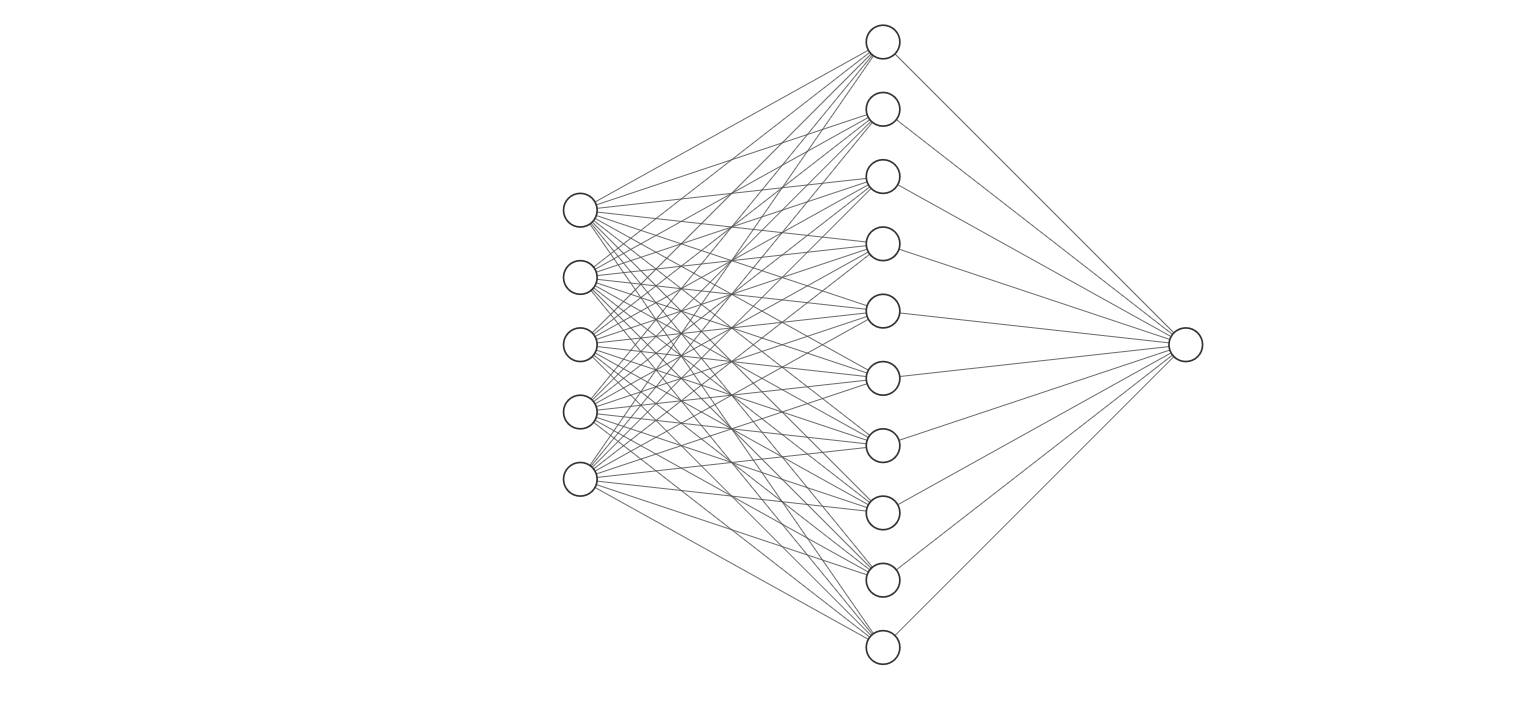
\includegraphics[width=0.9\textwidth]{nn.png}
		\caption{神经网络结构图}
	\end{figure}
	\begin{figure}[!h]
		\centering 
		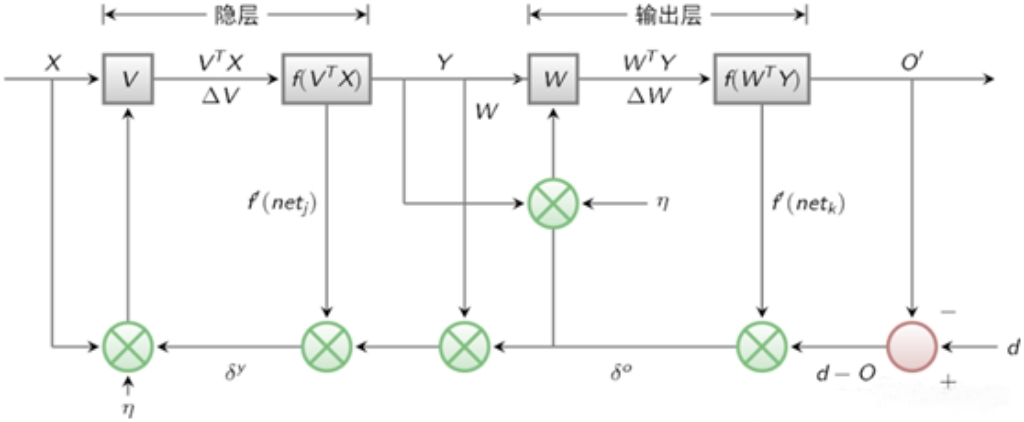
\includegraphics[width=0.7\textwidth]{nn流程图.jpg}
		\caption{神经网络流程图(该图源自网络)}
	\end{figure}
	
	首先把数据进行归一化处理
	\begin{equation}
		x_i=-1+2\times\frac{x_i-x_{imin}}{x_{imax}-x_{imin}}
	\end{equation}
	其中$x_{imax}$和$x_{imin}$是原所有$x_i$中的最大和最小值。
	
	在输入$X=(x_1,x_2,x_3,x_4,x_5)$到隐层的变换中,我们采用矩阵线性变化,通过$5\times n$的矩阵转化入隐层的$n$个神经元。
	即第一个$f_1(x)=x$,从隐藏层到输出层,采用传输函数输出。传输函数取双极性sigmoid函数,即$f_2(x)=\frac{1-e^{-x}}{1+e^{-x}}$,下面写成$s(x)$。我们对数据的训练就是对于两个层间变换矩阵的系数优化。系数的优化我们通过样本信号输入后的输出与理想期望输出的误差进行反馈。
	
	\subsubsection{学习算法}
	我们定义输出误差
	\begin{equation}
		E=0.5(d-o)^2=\sum_{i=1}^n 0.5(d_i-o_i)^2
	\end{equation}
	展开到隐层后得到
	\begin{equation}
		E=\sum_{i=1}^n0.5\left[d_i-f\left(\sum_{j=1}^5w_{ji}y_j\right)\right]^2
	\end{equation}
	展开到输入层后为
	\begin{equation}
		E=\sum_{i=1}^n0.5\left\{d_i-f\left[\sum_{j=1}^5w_{ji}\left(\sum_{l=1}^5v_{lj}x_i\right)\right]\right\}^2
	\end{equation}
	我们采用梯度下降进行误差反馈
	\begin{equation}
		\Delta w_{ji}=-\eta\frac{\partial E}{\partial w_{ij}}
	\end{equation}

	\begin{equation}
		\Delta v_{lj}=-\eta\frac{\partial E}{\partial v_{lj}}
	\end{equation}
	
	具体算法实现可以看所附的代码,最终我们训练得到的两层矩阵存在layer类型的自定义类当中。通过BP神经网络计算函数\verb|BPrun(lin_, lout_, vin_)|,我们可以利用输入层和输出层变换矩阵信息和输入得到输出。输入为几个变量组成的向量,由此我们成功构造了一个关于多种因素与乙醇转化率的关系网络。我们可以任意输入预设参数,在一定的范围内输出数据都有比较高的合理性。
	
	基于这样的神经网络架构理论,我们可以架构起A、B不同催化剂装料方式下有关五种变量与乙醇转化率和C4烯烃选择性的神经网络关系模型。
	
	\section{第三问}
	本题要求我们找到乙醇收率的最大值,即多元函数$y=f(x_1,x_2,x_3,x_4,x_5)$的峰值。在上题中我们找到了神经网络来代替构建这样一个函数,但是这个系统中的输入输出函数\verb|BPrun()|并不能简单地写出表达式,而且表达式的极值点计算难度非常大,很难得出完全精确的结论。因此在本题中我们依然采用启发式算法。
	对于这样一个复杂具体系统的最优解问题,我们尽量去寻找他的可行性局部最优解。可以权衡的方法有:爬山算法,模拟退火算法,遗传算法。
	鉴于爬山算法对多峰问题的局限性,模拟退火的高复杂度,本题采用了遗传算法进行最大值的搜索。
	\subsection{遗传算法}
	本题的算法实现使用了谢菲尔德大学提供的MATLAB遗传算法工具包,接下来详细解释一下其中的算法
	\begin{figure}[!h]
		\centering 
		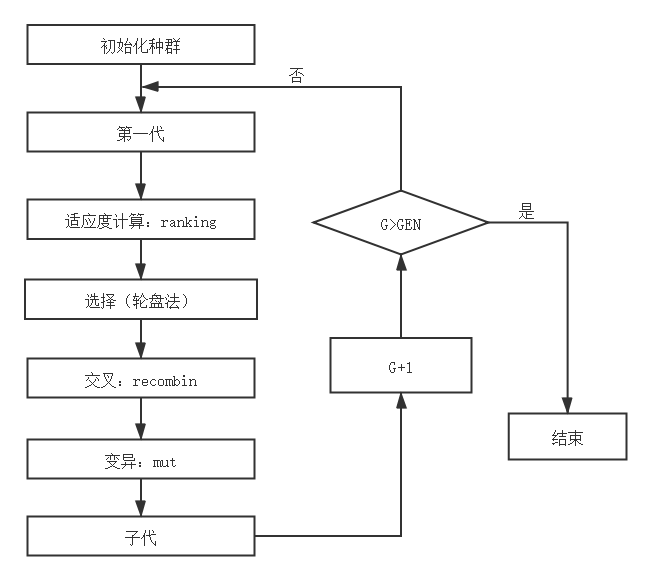
\includegraphics[width=0.8\textwidth]{遗传算法流程图.png}
		\caption{遗传算法流程图}
	\end{figure}
		
	建立神经网络时我们已经对自变量进行了归一化,于是个体的范围在$(-1,1)$之间。
	
	首先利用\verb|crtbp|函数进行种群初始化,其中个体基因由随机函数生成,用二进制串进行表示,可以使用\verb|bs2rv|函数转换为十进制。
	
	接下来确定基因的编码方式,我们采用格雷码编码,这种方式能把错误最小化,具体的编码方式用以下流程递归:1位格雷码有两个码字,$(n+1)$位格雷码中的前$2n$个码字等于$n$位格雷码的码字,按顺序书写,加前缀0,$(n+1)$位格雷码中的后$2n$个码字等于$n$位格雷码的码字,按逆序书写,加前缀1,$(n+1)$位格雷码的集合 = $n$位格雷码集合(顺序)加前缀$0+n$位格雷码集合(逆序)加前缀1。
	
	完成编码后我们要进行适应度计算的确立,我们利用ranking函数与神经网络构建BPrun函数进行适应度的计算排序,为之后的子代生成(交叉,变异)做准备。接下来要淘汰种群中的一部分,我们采用轮盘赌方法。上述ranking函数可以把适应性数值化,我们利用适应性的相对大小作为该种群存活下来的相对概率。
	
	而产生子代的过程要经过交叉和变异。对于交叉,我们采用均匀交叉,两个配对个体的每个基因座上的基因都以相同的交叉概率进行交换,从而形成两个新个体。具体为代码中的recombin函数。对于变异,我们采用均匀变异,分别用符合某一范围内均匀分布的随机数,以某一较小的概率来替换个体编码串中各个基因座上的原有基因值。由此我们产生子代并且插入原来的种群中,成为新的一代。如此反复,直到总代数G达到我们需求的次数。这便是我们采用的遗传算法的相关原理。
	\subsection{优化模型}
	延续前变量和关系假设,在该问中我们要选择合适的催化剂组合与温度,使得烯烃收率尽可能高。催化剂组合与温度为影响乙醇转化率和C4烯烃选择性的自变量,它们之间的关系已由神经网络确定。要使收率较高,那这就是以$(x_1,x_2,x_3,x_4,x_5)$为决策变量,以收率尽量高为目标的优化模型。目标如下:
	\begin{equation}
		\max PY=CR\times ST
	\end{equation}

	关系式由神经网络模型分析给出。而关于决策变量,限于实验条件限制,我们根据假设,即以表中数据阈值为其约束范围。由于装料方式A与B的不同,两者模型(关系式)不同,数据不同,约束条件也会不同。关于五个决策变量的约束条件为
	\begin{equation}
		A:\left\{\begin{array}{l}
			\begin{aligned}
				250&\leq x_1\leq 450 \\
				100&\leq x_2\leq 400 \\
				0.5&\leq x_3\leq 2\\
				0.5&\leq x_4\leq 5\\
				0.3&\leq x_5\leq2.1
			\end{aligned}
		\end{array}\right.
	\end{equation}

	\begin{equation}
		B:\left\{\begin{array}{l}
			\begin{aligned}
				250&\leq x_1\leq 400 \\
				20&\leq x_2\leq 200 \\
				x_3&=1\\
				x_4&=1\\
				0.9&\leq x_5\leq2.1
			\end{aligned}
		\end{array}\right.
	\end{equation}
	
	\newpage
	利用遗传算法运行5次,每次运行结果的较优解如下所示:
	\begin{table}[!h]
		\centering
		\caption{假设范围内催化剂组合与温度的选择}
		\begin{tabular}{|c|c|c|c|c|c|c|}
			\hline
			装料方式               & 温度    & 催化剂质量和 & 装料比 & Co负载量 & 乙醇浓度  & C4烯烃收率 \\ \hline
			\multirow{5}{*}{A} & 430.7 & 399.0  & 1.59           & 2.48  & 0.781 & 0.6982 \\ \cline{2-7} 
			& 433.0 & 399.4  & 1.61           & 2.19  & 0.394 & 0.6779 \\ \cline{2-7} 
			& 429.5 & 391.3  & 1.88           & 2.35  & 0.310 & 0.7340 \\ \cline{2-7} 
			& 434.2 & 396.8  & 1.97           & 2.34  & 0.420 & 0.7541 \\ \cline{2-7} 
			& 430.3 & 395.1  & 1.89           & 1.94  & 0.302 & 0.7748 \\ \hline
			\multirow{5}{*}{B} & 395.7 & 178.4  & 1.00           & 1.00  & 2.095 & 0.2513 \\ \cline{2-7} 
			& 397.9 & 163.3  & 1.00           & 1.00  & 1.982 & 0.2522 \\ \cline{2-7} 
			& 397.3 & 164.5  & 1.00           & 1.00  & 2.099 & 0.2580 \\ \cline{2-7} 
			& 390.8 & 175.2  & 1.00           & 1.00  & 2.088 & 0.2328 \\ \cline{2-7} 
			& 394.1 & 173.6  & 1.00           & 1.00  & 2.099 & 0.2464 \\ \hline
		\end{tabular}
	\end{table}

	综合考量,选择装料方式A,当自变量组合$(x_1,x_2,x_3,x_4,x_5)=(430.3,395.1,1.89,1.94,0.302)$时收率较高,为$0.7748$。
	
	要使温度低于350度时收率尽可能高,与前情况类似,仅需再加入一个约束函数,即$x_1\leq 350$。同样利用遗传算法运行五次,每次运行结果的较优解如下所示:
	\begin{table}[!h]
		\centering
		\caption{低于350度时催化剂组合与温度的选择}
		\begin{tabular}{|c|c|c|c|c|c|c|}
			\hline
			装料方式               & 温度    & 催化剂质量和 & 装料比 & Co负载量 & 乙醇浓度  & C4烯烃收率 \\ \hline
			\multirow{5}{*}{A} & 349.6 & 247.3  & 1.99           & 4.09  & 1.608 & 0.2304 \\ \cline{2-7} 
			& 349.8 & 235.7  & 2.00           & 4.51  & 1.757 & 0.2201 \\ \cline{2-7} 
			& 343.3 & 248.0  & 1.98           & 3.37  & 1.255 & 0.2283 \\ \cline{2-7} 
			& 336.9 & 240.4  & 1.95           & 3.30  & 1.223 & 0.2152 \\ \cline{2-7} 
			& 349.5 & 231.7  & 1.99           & 4.21  & 1.707 & 0.2240 \\ \hline
			\multirow{5}{*}{B} & 349.0 & 137.4  & 1.00           & 1.00  & 2.090 & 0.0892 \\ \cline{2-7} 
			& 339.8 & 128.6  & 1.00           & 1.00  & 2.092 & 0.0692 \\ \cline{2-7} 
			& 349.5 & 136.2  & 1.00           & 1.00  & 2.093 & 0.0904 \\ \cline{2-7} 
			& 349.4 & 136.0  & 1.00           & 1.00  & 2.088 & 0.0898 \\ \cline{2-7} 
			& 349.1 & 137.4  & 1.00           & 1.00  & 2.087 & 0.0894 \\ \hline
		\end{tabular}
	\end{table}

	综合考量,在温度要求低于350度时,选择装料方式A,当自变量组合$(x_1,x_2,x_3,x_4,x_5)=(349.6,247.3,1.99,4.09,1.608)$时收率较高,为$0.2304$。
	\section{第四问}
	在第三问中,我们得到了在我们建立的神经网络模型下使收率尽可能高的温度与催化剂组合。但由于我们的模型是通过数学模型得到的,它与实际情况不一定相符,所以在该问设计五个实验时,我们的实验目的便是要检验我们得到的温度与催化剂组合是否相对优于其他组合使收率尽可能高。同时出于用实验帮助我们更好地判断各因素的影响的考虑,我们要用到控制变量的思想去设计,即通过更改自变量组合的一个变量去设计实验。
	
	由于我们设计的实验次数为5次,首先我们要验证模型与实际情况是否相贴合,即要对上题所得的最优组合进行实验操作,得到收率数据,与其计算值比较,看计算值与实际值是否存在较大误差,以判断神经网络模型是否成立。而另一方面就是验证所求是否为较优解,即判断模型和算法是否同时在现实情况下成立,这里用到控制变量。按理温度与催化剂组合的自变量有6个,但是由相关性分析和上述算法结论,我们认为装料方式不同与收率结果差异较大,收率与装料比相关性不存在较大关联,所以不考虑这两个变量的更改,对其余变量作一定程度更改,确立总的5组实验方案如下:
	\begin{table}[!h]
		\centering
		\caption{实验方案设计}
		\begin{tabular}{|c|c|c|c|c|c|c|}
			\hline
			实验方案 & 装料方式 & 温度    & 催化剂质量和 & 装料比  & Co负载量 & 乙醇浓度  \\ \hline
			1    & A    & 430.3 & 395.1  & 1.89 & 1.939 & 0.302 \\ \hline
			2    & A    & 420.3 & 395.1  & 1.89 & 1.939 & 0.302 \\ \hline
			3    & A    & 430.3 & 385.1  & 1.89 & 1.939 & 0.302 \\ \hline
			4    & A    & 430.3 & 395.1  & 1.89 & 2.039 & 0.302 \\ \hline
			5    & A    & 430.3 & 395.1  & 1.89 & 1.939 & 0.312 \\ \hline
		\end{tabular}
	\end{table}
	\section{算法分析和优化}
	\subsection{可行性分析}
	在问题求解过程中,我们用了回归模型和相关性分析的相关模型,在做这些模型时,我们都做了显著性检验,显著性检验的一系列系数确保了我们的回归和相关性分析所得结果是可靠的。
	
	对于神经网络,我们将一系列实验数据代入该模型后,系统输出与表格内实验结果基本符合,误差较小,说明神经网络模型可行。
	
	最后要验证遗传算法的可行性,即要在模型上证明我们得到的较优解确实是在烯烃收率上是优越的。在此参考第四问的实验方案,将第四问方案代入神经网络模型,得到的烯烃收率计算值为$(0.7748,0.7334,0,6133,0.7193,0.6922)$,这说明在我们的模型理论上实验方案1在控制变量时确实较优,遗传算法可行。
	
	至此,我们对本文中所用的所有模型算法完成了可行性分析。
	
	\subsection{优缺点分析}
	\subsubsection{优点}
	\begin{itemize}
		\item[(1)]总体而言,我们将本道化学问题背后的数学本质挖掘出来,建立了严谨合理的数学模型。文章逻辑清晰,各小节之间关系紧密、层层递进,逐步深入进行探讨。
		\item[(2)]对于各个问题,我们都采用了针对性的方法进行分析解决,各方法均有足够的数学理论进行支撑,并且不同算法得到的结果相互佐证,证明了本篇文章的科学性和合理性。
		\item[(3)]本篇文章综合了回归分析、神经网络算法、遗传算法等多种数学方法,并在适当的场景有效地满足了各问题的需求。
	\end{itemize}
	
	\subsubsection{缺点}
	\begin{itemize}
		\item[(1)]数据量较少是本次建模中我们面临的最大的问题之一,我们在第二部分建立的神经网络模型也因此无法进行足够数据量的训练,无法确保模型的泛化能力。
		\item[(2)]在第三部分的遗传算法设计中,由于只进行了部分随机搜索,虽然得到的几组局部最优解的结果较为相近,但我们仍然无法确保此处解是最优解。
		\item[(3)]由于数据量和算法的限制,我们无法确定各变量之间的具体关系表达式,因此在确定实验最适条件和设计实验的过程中,存在一定的误差。
	\end{itemize}

	\subsection{改进策略}
	\begin{itemize}
		\item[(1)]改进神经网络的学习算法,增强模型的学习和泛化能力,在较少数据量的情况下得到较优解。
		\item[(2)]加大遗传算法的搜索范围并拓展搜索深度,希望得到更准确的局部最有解。
		\item[(3)]可以探究变量间更多的函数拟合关系,得到更加具体的影响关系,从而更加利于实际实验。
	\end{itemize}

	\section{结语}
	在本题的探究过程中,我们建立了合理的数学模型,并针对题目的要求设计了具体算法,总体而言可以较好地满足题目的要求,解决了相应的问题,并且有一定的实际应用价值。对于探究过程中出现的问题,我们也进行了分析并提出了相应的解决策略,恳请批评指正!
	
	\begin{thebibliography}{10}  
		\bibitem{ref1}简书,https://www.jianshu.com/p/ae5157c26af9
		\bibitem{ref2}CSDN,神经网络学习之BP神经网络,https://blog.csdn.net/u013007900/article/details/50118945
	\end{thebibliography}
	
\end{document}

